\chapter{Characteristics of GWs excited by propagating tropopause depressions in ground-based lidar observations}
\label{cha:lidar}
% Lidar observations in Q3D simulations are not useful / used y position 1 instead on npy/2!! --> use local 2D simulations for analysis of these plots (eventually conduct constant wind simulations again)
% radiances from the Cross-Track Infrared Sounder (CrIS) on the Suomi National Polar-Orbiting Partnership (NPP) satellite that launched on October 2011 as the first stage of the Joint Polar Satellite System (JPSS; Goldberg et al. 2013)
% COSMIC satellite

Observations of GWs in the upper atmosphere (stratosphere and MLT) are sparse. Only a small number of satellite instruments provide temperature measurements in this altitude range applicable for the detection of GWs.For example, the High Resolution Dynamics Limb Sounder (HIRDLS) was only active between 2005 and 2008 (\cite[]{gille_high_2008}). The Sounding of the Atmosphere using Broadband Emission Radiometry (SABER) is part of the Thermosphere-Ionosphere-Mesosphere Energetics and Dynamics (TIMED) mission and still operational, but only provides continuous measurements for the the latitude range \SI{50}{\degree N}-\SI{50}{\degree S} (\cite[]{mlynczak_energetics_1997} and \cite[]{ern_gracile_2018}). Other instruments are the Cross-Track Infrared Sounder (CrIS) on the Suomi National Polar-Orbiting Partnership (NPP) satellite that launched on October 2011 (\cite[]{goldberg_joint_2013}) or the nadir-sounding Atmospheric Infrared Sounder (AIRS) on board of NASA's Aqua satellite (e.g \cite[]{eckermann_stratospheric_2019}, \cite[]{hindley_gravity_2019} or \cite*[]{hindley_18year_2020}). In the case of AIRS, measurements are available globally, but the temporal resolution is coarse, because each location is only observed twice a day. In addition, the instrument is sensitive to just a portion of the GW spectrum due to the so-called "observational filter" of the instrument properties (e.g. \cite[]{preusse_space-based_2002} or \cite[]{alexander_recent_2010}). Observations of the other satellite instruments are even more constrained. 

Vertical temperature profiles from ground-based Lidar stations are the only alternative available on a regular basis. They provide much higher vertical and temporal resolution at the cost of being limited to a single location (point observation), often night-time and clear sky conditions. The analysis of GWs in these measurements is challenging and at a certain point not possible without consulting additional information from other observations or model data. Thus, it is the goal of this chapter to provide a basis for identifying NOGWs from tropopause folds in these ground-based measurements and tackle the fifth research question of this thesis:
%
\begin{tcolorbox}[]
    (R5) Can NOGWs from propagating tropopause depressions be identified in ground-based lidar observations?
\end{tcolorbox}
% Thus, representative patterns from theory or idealized studies are highly appreciated for their intepretation and
Though the proposed excitation mechanism of these NOGWs is supposed to mimic the excitation of MWs over topography, their appeareance in lidar observations might differ due to the propagation of their source. Therefore, section \ref{sec:lidOb-idealized} first deals with the question of how GWs generated by propagating tropopause depressions show up in vertical timeseries and how they could be interpreted utilizing the idealized simulations described in previous chapters.
Subsequently, section \ref{sec:lidOb-coral} presents two measurements of the Rayleigh Lidar CORAL (chapter \ref{sec:coral}) that show similar signatures as the idealized simulations. A first interpretation based on ERA5 reanalysis data is discussed, but it can be anticipated that further tools like for example high resolution simulations are needed to reach a conclusive interpretation. 

\section{Lidar observations in idealized numerical simulations}
\label{sec:lidOb-idealized}
% The goal of the following analysis is

% High resolution vertical time series at multiple locations were retrieved from the idealized numerical simulations discussed in previous chapters.

Wave properties of stationary mountain waves are somewhat unfavorable from a lidar observation point of view. In purely steady flow conditions, their horizontal phase speed vanishes ($c_{px}=0$) together with the ground-based frequency ($\omega$=0). As a result, phase lines in vertical time series of ground-based lidar observations appear horizontal and one can only derive the vertical wavelength $\lambda_z$ from the observations, but misses information on horizontal scales (e.g. \cite[]{dornbrack_interpretation_2017} or \cite[]{reichert_highcadence_2021}). Section \ref{sec:resultsQ3D} showed that NOGWs from a propagating source might develop similar properties as stationary MWs, but within the reference frame moving with their source. Figure \ref{fig:lidar_sim} illustrates how this alters their appearance in vertical time series as they would be observed by a ground-based lidar. As discussed in section \ref{sec:resultsQ3D}, the wave forcing of a trough moving with $c_{tf}$ (\ref{fig:lidar_sim}b) for a certain point in time can be reproduced by a stationary trough with a wind profile reduced by $c_{tf}$ (Figure \ref{fig:lidar_sim}c). However, phase lines in the vertical time series differ significantly and show an upward (downward) tilt for a source moving in the same (opposite) direction as the background wind (Figure \ref{fig:lidar_sim}d, downward tilt not shown). The similar feature can be observed for a more realistic wind profile with a tropopause jet and a polar night jet in Figure \ref{fig:lidar_sim}e and f (the reference simulation of chapter \ref{sec:resultsQ3D}). Does this allow for a derivation of horizontal wave properties? Yes and no! Clearly, tilted phase lines enable the quantification of a ground-based period $T$ from the vertical time series, but linking this period to wave properties depends on the wave source and atmospheric background conditions. Multiple phenomena could explain upward tilted phase lines in lidar observations, so their intepretation requires additional knowledge on the prevailing processes and synoptic situation. Examples are:
%  so by considering lidar observations only, upward tilted phase lines could for example be attributed
% \cite[]{ern_absolute_2004}

\begin{itemize}
    \item downward propagating wave packets caused by reflection or wave breaking in the upper atmosphere which excites secondary waves that travel up and down from their source region (\cite[]{dornbrack_interpretation_2017} and \cite[]{vadas_mechanism_2003}).
    % fishbone pattern

    \item transient background conditions. Mainly in the form of a varying wind speed and wind direction, but also in the context of a transient lower boundary (topography). The latter is visible in Figure \ref{fig:lidar_sim}b in the context of the spin up process (rising topography) of the simulation which implies slightly downward tilted phase lines within the first \SI{50}{\hour} of the simulation.

    \item a GW source moving in the same direction as the background wind as illustreated in Figure \ref{fig:lidar_sim}d and \ref{fig:lidar_sim}f.
\end{itemize}

\begin{figure*}[tbp]
    \centering
    \includegraphics[width=0.95\textwidth]{figures_lidar/lidana_th.png}
    \caption{Shown are vertical cross-sections (a,c,e) after $t$=\SI{72}{\hour} with vertical wind profiles in purple and vertical time series (b,d,f) at the outlined position for three different simulations. The first simulation (a,b) features a stationary obstacle at the lower boundary and a constant wind profile. In the second simulation (c,d) the trough moves to the right with a constant speed $c_{tf}$=\SI{13.88}{\meter \per \second} and the wind is increased by the same amount. The last simulation (e,f) represents the reference simulation of the sensitivity analysis in section \ref{sec:resultsQ3D} with a more realistic stratospheric winter time wind profile. The assessment of $\lambda_z$ and period $T$ from the vertical time series is labeled in (d), two consecutive $\lambda_x$ are labeled in (c). Contour lines represent constant potential temperature and the amplitude of the lower boundary is scaled by a factor of 5.}
    \label{fig:lidar_sim}
\end{figure*}

For this work we continue with the last explanation and focus on the GW characterization for the simplified case of a constant wind profile shown in Figure \ref{fig:lidar_sim}c and \ref{fig:lidar_sim}d following the terminology and derivations of \textcite[]{gill_atmosphere-ocean_1982}, \textcite[]{fritts_gravity_2003} or \textcite[]{dornbrack_interpretation_2017}. To recap, a constant stratification with $N=\SI{0.02}{\per \second}$ was used for all simulations starting at the tropopause simplifying the dispersion relation for Boussinesq flows to
\begin{equation}
    \hat{\omega}^2 = N^2 \frac{k^2}{k^2+m^2} + f^2 \frac{m^2}{k^2+m^2}
    \label{equ_lid:dispersion}
    % observed waves obey a dispersion relation for internal Boussinesq
    % Alhough variations in density are the very essence of buoyancy, they are neglected everywhere in the Boussinesq equations “except in so far as they modify the action of gravity” (Rayleigh, 1916), i.e., the density is assumed to be constant except in the buoyancy force
    % by applying a peak finding algorith to the vertical profile and additionally a time span $T$ applying the same algorithm along the time axis
\end{equation}
with $\hat{w}$ being the intrinsic frequency and $f=$ \SI{-1.195e-4}{\per \second} the Coriolis parameter to consider the influence of Earth's rotation at a latitude of $55\degree$S. A constant background wind leads to a ground-based frequency
\begin{equation}
    \omega = \hat{\omega} + uk,
    % w = \hat{w} + uk = \frac{Nk}{\sqrt{k^2+m^2}}.
    \label{equ_lid:omega}
\end{equation}
and, in addition, \textcite{gill_atmosphere-ocean_1982} defines the useful aspect ratio
\begin{equation}
    \alpha = \frac{\text{vertical scale}}{\text{horizontal scale}} = \frac{\lambda_z}{\lambda_x} = \sqrt{\frac{\hat{\omega}^2-f^2}{N^2-\hat{\omega}^2}},
    \label{equ_lid:alpha}
\end{equation}
which simplifies the approximation of $\hat{\omega}$ for the relevant hydrostatic rotating wave regime to
\begin{equation}
    \hat{\omega}^2 \approx f^2 + N^2 \alpha^2.
    \label{equ_lid:omega_simp}
\end{equation}
As labeled in Figure \ref{fig:lidar_sim}d, the vertical distance between troughs or ridges in the vertical time series yields the vertical wavelength $\lambda_z=\SI{9.25}{\kilo \meter}$ and wavenumber $m$, the horizontal distance at \SI{40}{\kilo \meter} provides a period $T=\SI{13.92}{\hour}$ and ground-based frequency $\omega$. How can this frequency be interpreted? \textcite[]{dornbrack_interpretation_2017} clarify that in the presence of a background wind this question can only be answered by consulting further information or by proceding with assumptions. For the case of a propagating tropopause depression we can assume a stationary wave field within a reference frame that propagates with the depression. Then the tilt of the phase lines within the lidar observation depends on the propagation speed of the GW source and the horizontal wavelength $\lambda_x$. A constant propagation speed $c_{tf}$=\SI{13.88}{\meter \per \second} leads to $\lambda_x = T \cdot c_{tf}$= \SI{695}{\kilo \meter}, which is in the range of wavelengths labeled in the vertical cross-section (Figure \ref{fig:lidar_sim}c) at the same height with $\lambda_x$=\SI{525}{\kilo \meter} - \SI{712}{\kilo \meter}. The ratio of $\lambda_x$ and $\lambda_z$ gives $\alpha=0.0133$ and it is possible to define the angle formed between lines of constant phase and the z-axis in real space
\begin{equation}
    \phi = \tan^{-1}(\frac{\lambda_x}{\lambda_z})=89.24\degree.
    \label{equ_lid:phi}
\end{equation}
From equation \ref{equ_lid:omega_simp} $\hat{\omega}\approx$ \SI{2.92e-4}, so $\hat{\omega}$ is of $\mathcal{O}(f)$ and $\hat{\omega} \geq f$, which is in full compliance with the hydrostatic rotating wave regime described by \textcite[]{gill_atmosphere-ocean_1982}. It follows the intrinsic horizontal group velocity
\begin{equation}
    c_{gx} \approx \frac{N^2 \alpha}{m \sqrt{f^2+N^2 \alpha^2}} \approx \SI{-26.9}{\meter\per\second} 
    \label{equ_lid:cgh}
    % (phase propagation against the background wind results in a negative horizontal scale $k$ and, thus, negative $\alpha$)
\end{equation}
with a negative $m$ for upward propagating waves and the vertical group velocity
\begin{equation}
    c_{gz} \approx -\alpha c_{gx} \approx \SI{0.36}{\meter\per\second}
    \label{equ_lid:cgz}
\end{equation}
Again, this is in compliance with inertia-gravity waves in the hydrostatic rotating wave regime, where $c_{gx}$ does not compensate the background wind forcing. Knowing $U=\SI{45}{\meter\per\second}$ allows the calculation of $U_{MW}=U-c_{tf}=\SI{31.12}{\meter\per\second}>\lvert c_{gx} \rvert$ indicating a leeward extend of the GWs with respect to the propagating tropopause fold. Considering the superimposed propagation with the fold the ground-based or extrinsic group velocity is $c_{Gx}=U+c_{gx}=\SI{18.1}{\meter\per\second}$ and following the assumptions above the ground-based horizontal phase speed has to be identical to the speed of the depression ($c_{Px} = c_{tf}$). \\
The vertical propagation of the GWs is independent of the background wind. According to $c_{gz}$ in Equation \ref{equ_lid:cgz}, it takes approximately \SI{31}{\hour} until the GWs reach an altitude of \SI{40}{\kilo\meter} above the tropopause, but $c_{gz}$ is very sensitive to derived horizontal and vertical wavelengths. A $\lambda_x = \SI{525}{\kilo\meter}$ (lower limit based on Figure \ref{fig:lidar_sim}c) with the same $\lambda_z$ already results in \SI{22.6}{\hour} and higher $\lambda_z$ further increases $c_{gz}$. The vertical timeseries in Figure \ref{fig:lidar_sim}b for the stationary tropopause fold provides a consistent picture. Maximum amplitudes at \SI{40}{\kilo\meter} appear roughly 20-\SI{30}{\hour} after the completed spin up (continuous increase of tropopause fold depth during first \SI{12}{\hour} of the simulation).

% First of all, there have to be sufficiently large tropospheric winds perpendicular to the mountain ridge for excitation of MWs (e.g., Bramberger et al., 2017; Dörnbrack et al., 1999; Kaifler, Kaifler, et  al.,  2015). In addition, Dörnbrack et  al.  (1999) report that good excitation conditions prevail when the wind turns no more than 30° within the first 30 km. Monthly mean wind speeds in ERA5 data are at about 𝐴𝐴 15 ms−1 at surface level (500 m) at all times. The wind rotation within the first 30 km is <30° during the months from March to October with a surface level forcing between 240° and 280°. Thus, in the climatological mean MWs are excited and able to propagate deep into the middle atmosphere in the winter months. A strong wind rotation within the first 30 km of about 60° can only be observed in July 2020. At this time, we also find reduced GW energies at all altitude regions (see Figure 6). For upward propagation, the wind speed in the direction of wave propagation must not become zero as this would lead to wave breaking (Lindzen,  1981). Moreover, for deep vertical propagation, the MWs should not encounter turning levels where the intrinsic frequency approaches the buoyancy frequency (e.g., Schoeberl, 1985). These conditions occur in the core of the PNJ and filter horizontally short MWs or lead to evanescent modes tunneling through the PNJ (e.g., Mixa et al., 2021). Another obstacle for MWs is the stratospheric wind minimum where the waves' 𝐴𝐴𝐴𝐴′-amplitude may become equal to the horizontal wind speed causing wave breaking. This wind minimum can act as a valve for vertically propagating MWs (Kruse et al., 2016). Figure 10 reveals that low wind speeds at ∼25 km altitude occur from March to May. In the winter months, with positive temperature gradients (Figure 2) and large horizontal wind speeds (Figure 10) up to 50 km, generally good vertical propagation conditions can be expected. Above, shear instabilities and unstable lapse rates lead to wave dissipation. On the other hand, the mesosphere is the favorable region for the generation of secondary gravity waves (Heale et al., 2020; Kogure et al., 2020; Vadas & Becker, 2019; Vadas et al., 2018). Large contributions of apparently up- and downward propagating waves and reduced contributions of stationary waves (see Table 3) at mesospheric altitudes might indicate their existence above Río Grande.

\section{Potential signatures of NOGWs from propagating tropopause depressions in CORAL measurements}
\label{sec:lidOb-coral}
%
After a detailed investigation of the proposed excitation mechanism for NOGWs above tropopause folds through idealized numerical simulations, this section goes one step further and tries to identify the pattern of these GWs (discussed in the Section \ref{sec:lidOb-idealized}) in actual lidar measurements of the stratosphere and mesosphere. Ideally, this lidar station would be located within the latitude band of the PNJ around \SI{60}{\degree S} to ensure relevant excitation and propagation conditions. And it should be far away from orography to eliminate the superposition of MWs and NOGWs. Since 2018 the Compact Autonomous Rayleigh Lidar (CORAL) of the DLR conducts measurements at the southern tip of South America (\SI{53.79}{\degree S}) in Río Grande, Argentina (Section \ref{sec:coral}). It's automatic operation provides a unique dataset of observations within the relevant latitude band, but its proximity to the Andes Mountains is not a coincidence. It is a very appropriate location to study Earth's GW hot spot with large amplitude MWs (\cite[]{rapp_southtrac-gw_2021} or \cite[]{reichert_highcadence_2021}). As so often, reality is not ideal. Nevertheless, it might still be possible to identify signatures of NOGWs from propagating tropopause folds in these lidar measurements, even though MWs dominate CORAL's measurements. Hereafter, two CORAL observations are selected that show similar patterns as the vertical timeseries of the idealized simulations, more specifically, upward tilted phase lines. 

Figure \ref{fig:coral_2018} and Figure \ref{fig:coral_2020} show temperature measurements for a night in June 2018 and a night in August 2020. A background state $\bar{T}$ and perturbations $T'$ are obtained by applying a vertical highpass Butterworth filter with a cutoff wavelength of $\lambda_{z,cut}=\SI{20}{\kilo\meter}$. Though multiple studies suggest $\lambda_{z,cut}=\SI{15}{\kilo\meter}$ for MWs, we adapt to the results of \textcite[]{reichert_characterization_2022}, who discovered that more than \SI{50}{\percent} of the waves in the relevant CORAL dataset exhibit vertical wavelengths larger than \SI{16.5}{\kilo\meter}. Most likely, a result of the very strong horizontal winds of the PNJ above Río Grande in austral winter.
%%% first case (2018)
\begin{figure*}[tbp]
    \centering
    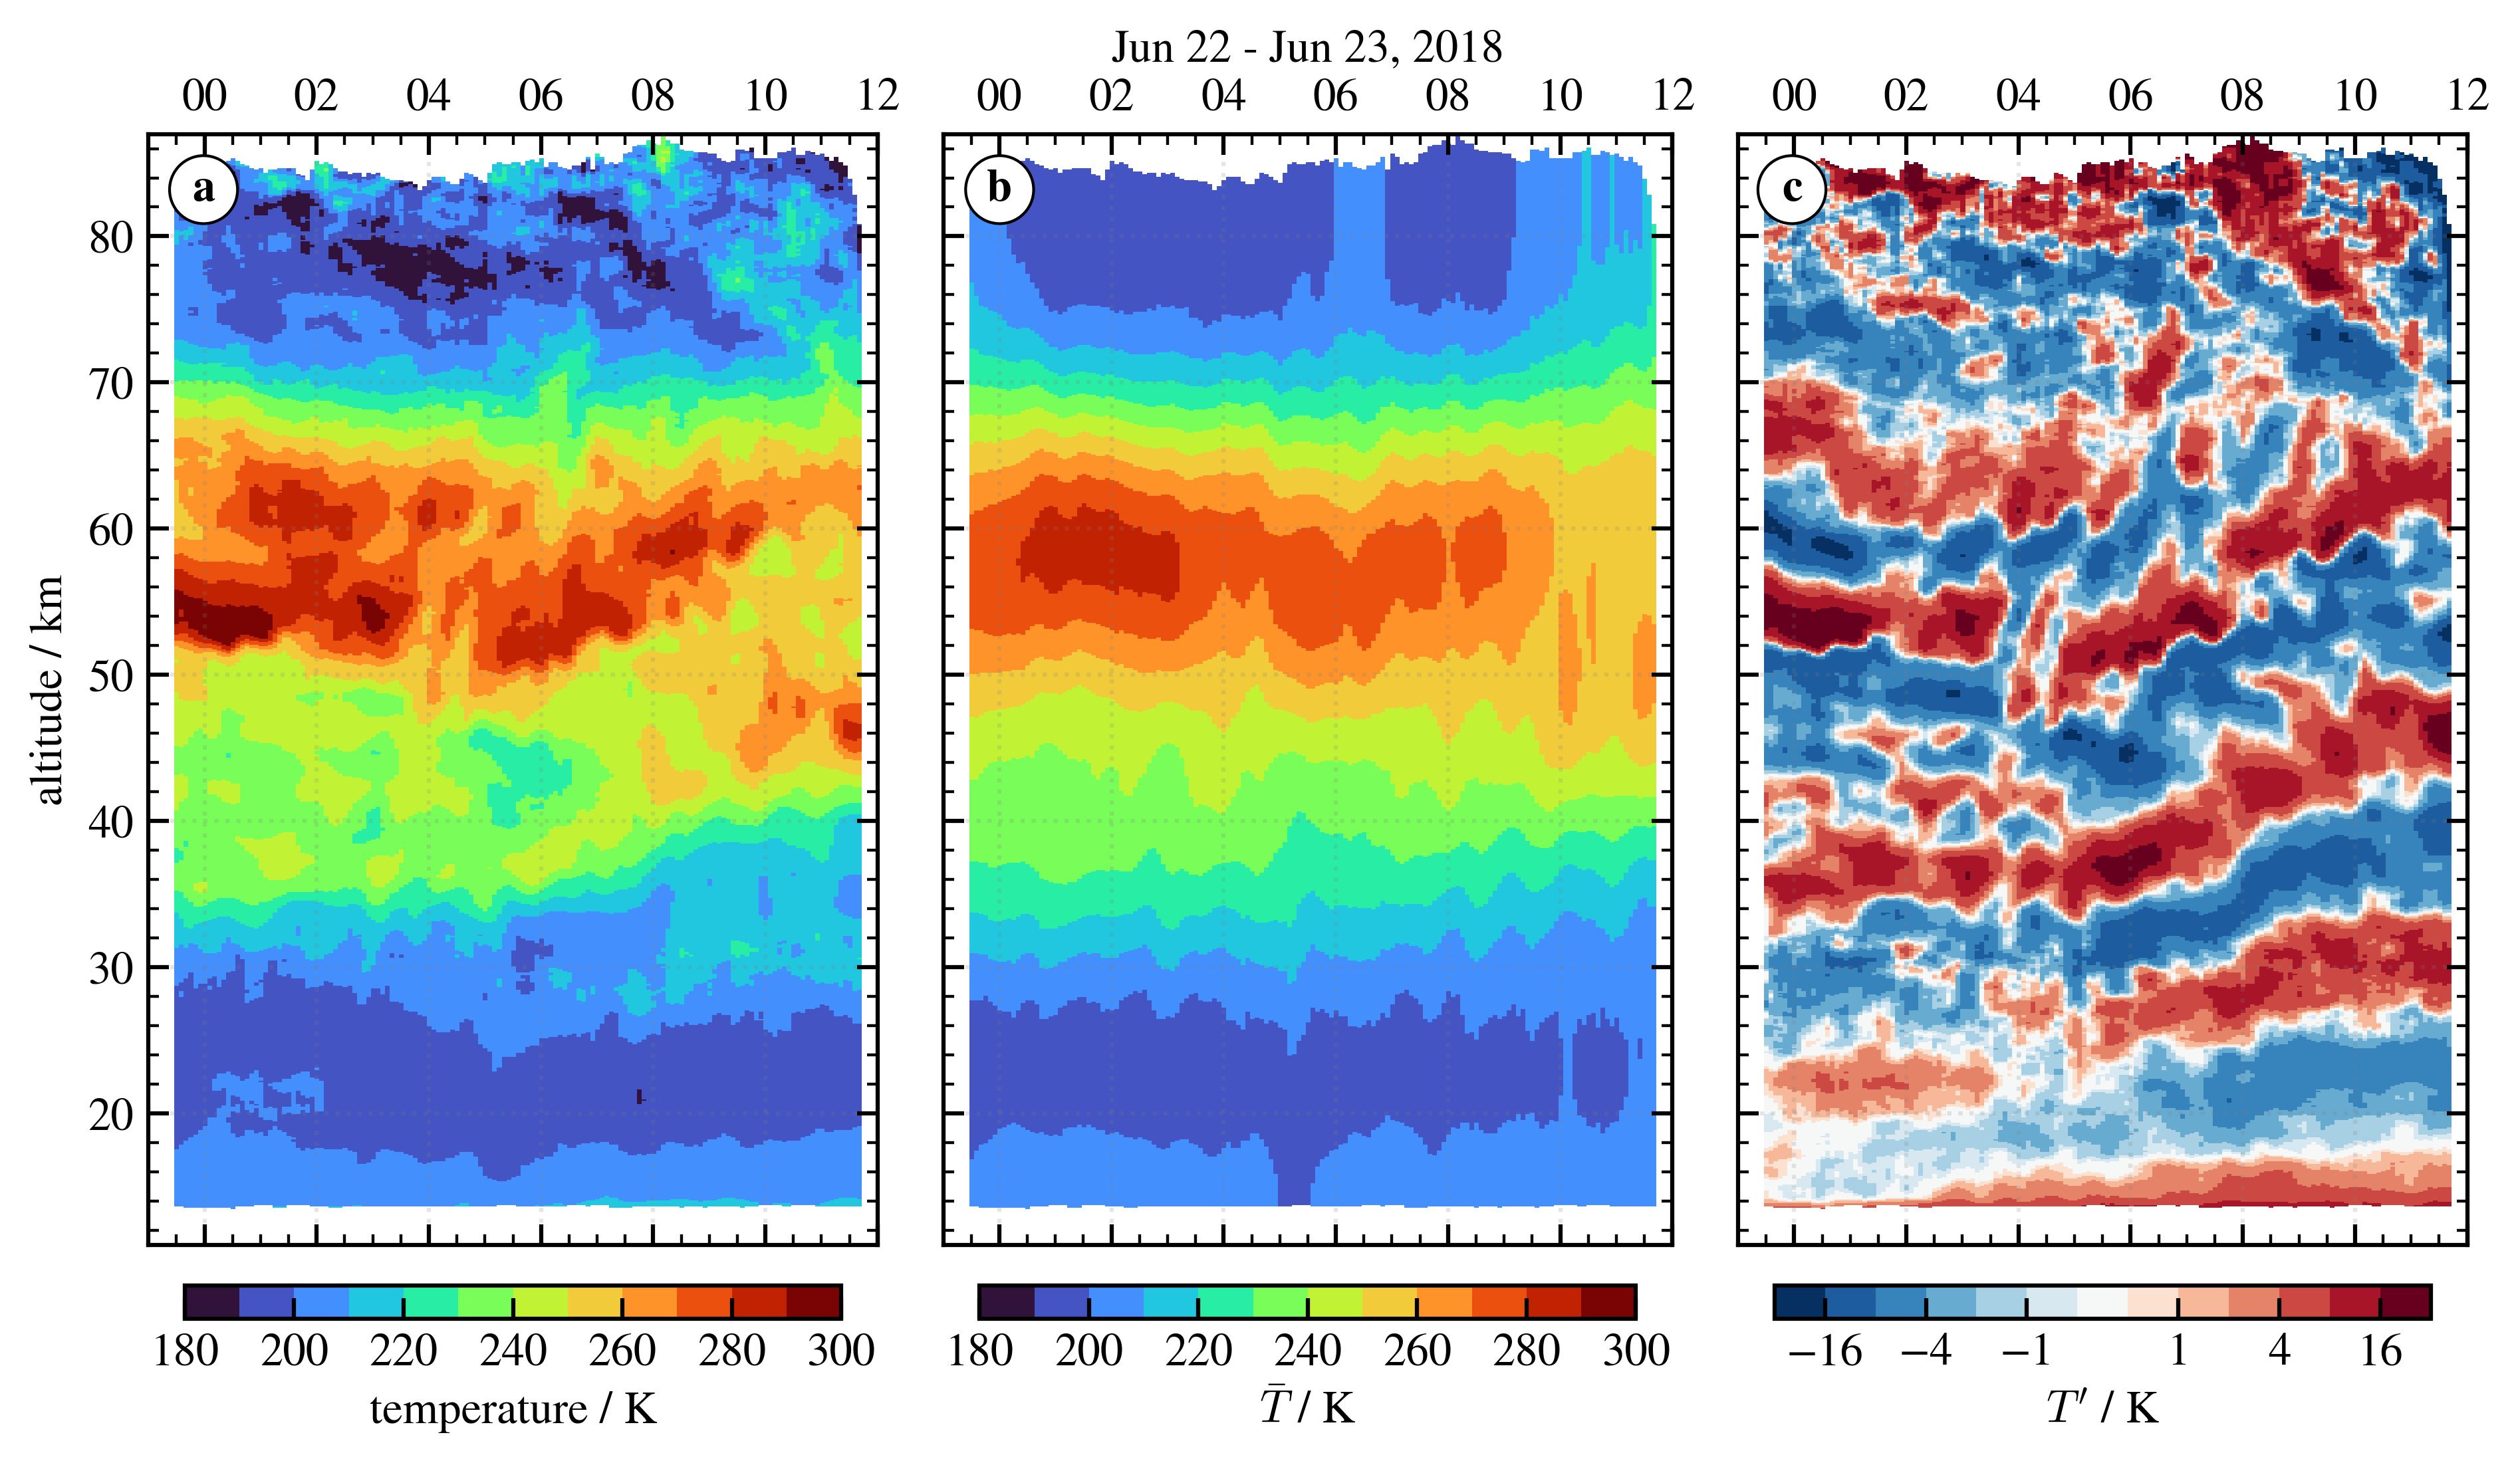
\includegraphics[width=0.9\textwidth]{figures_lidar/coral_event_20180622.png}
    \caption{Night-time temperature measurements of CORAL located in Río Grande, Argentina (\SI{53.79}{\degree S}, \SI{67.75}{\degree W}) from the 22nd to the 23rd of June 2018. Shown are retrieved temperature profiles (a), background temperature profiles $\bar{T}$ after applying a vertical high-pass Butterworth filter with a cutoff wavelength of $\lambda_{z,cut}=\SI{20}{\kilo\meter}$ (b) and temperature perturbations $T'=T-\bar{T}$ (c).}
    \label{fig:coral_2018}
\end{figure*}
%%% second case (2020)
\begin{figure*}[tbp]
    \centering
    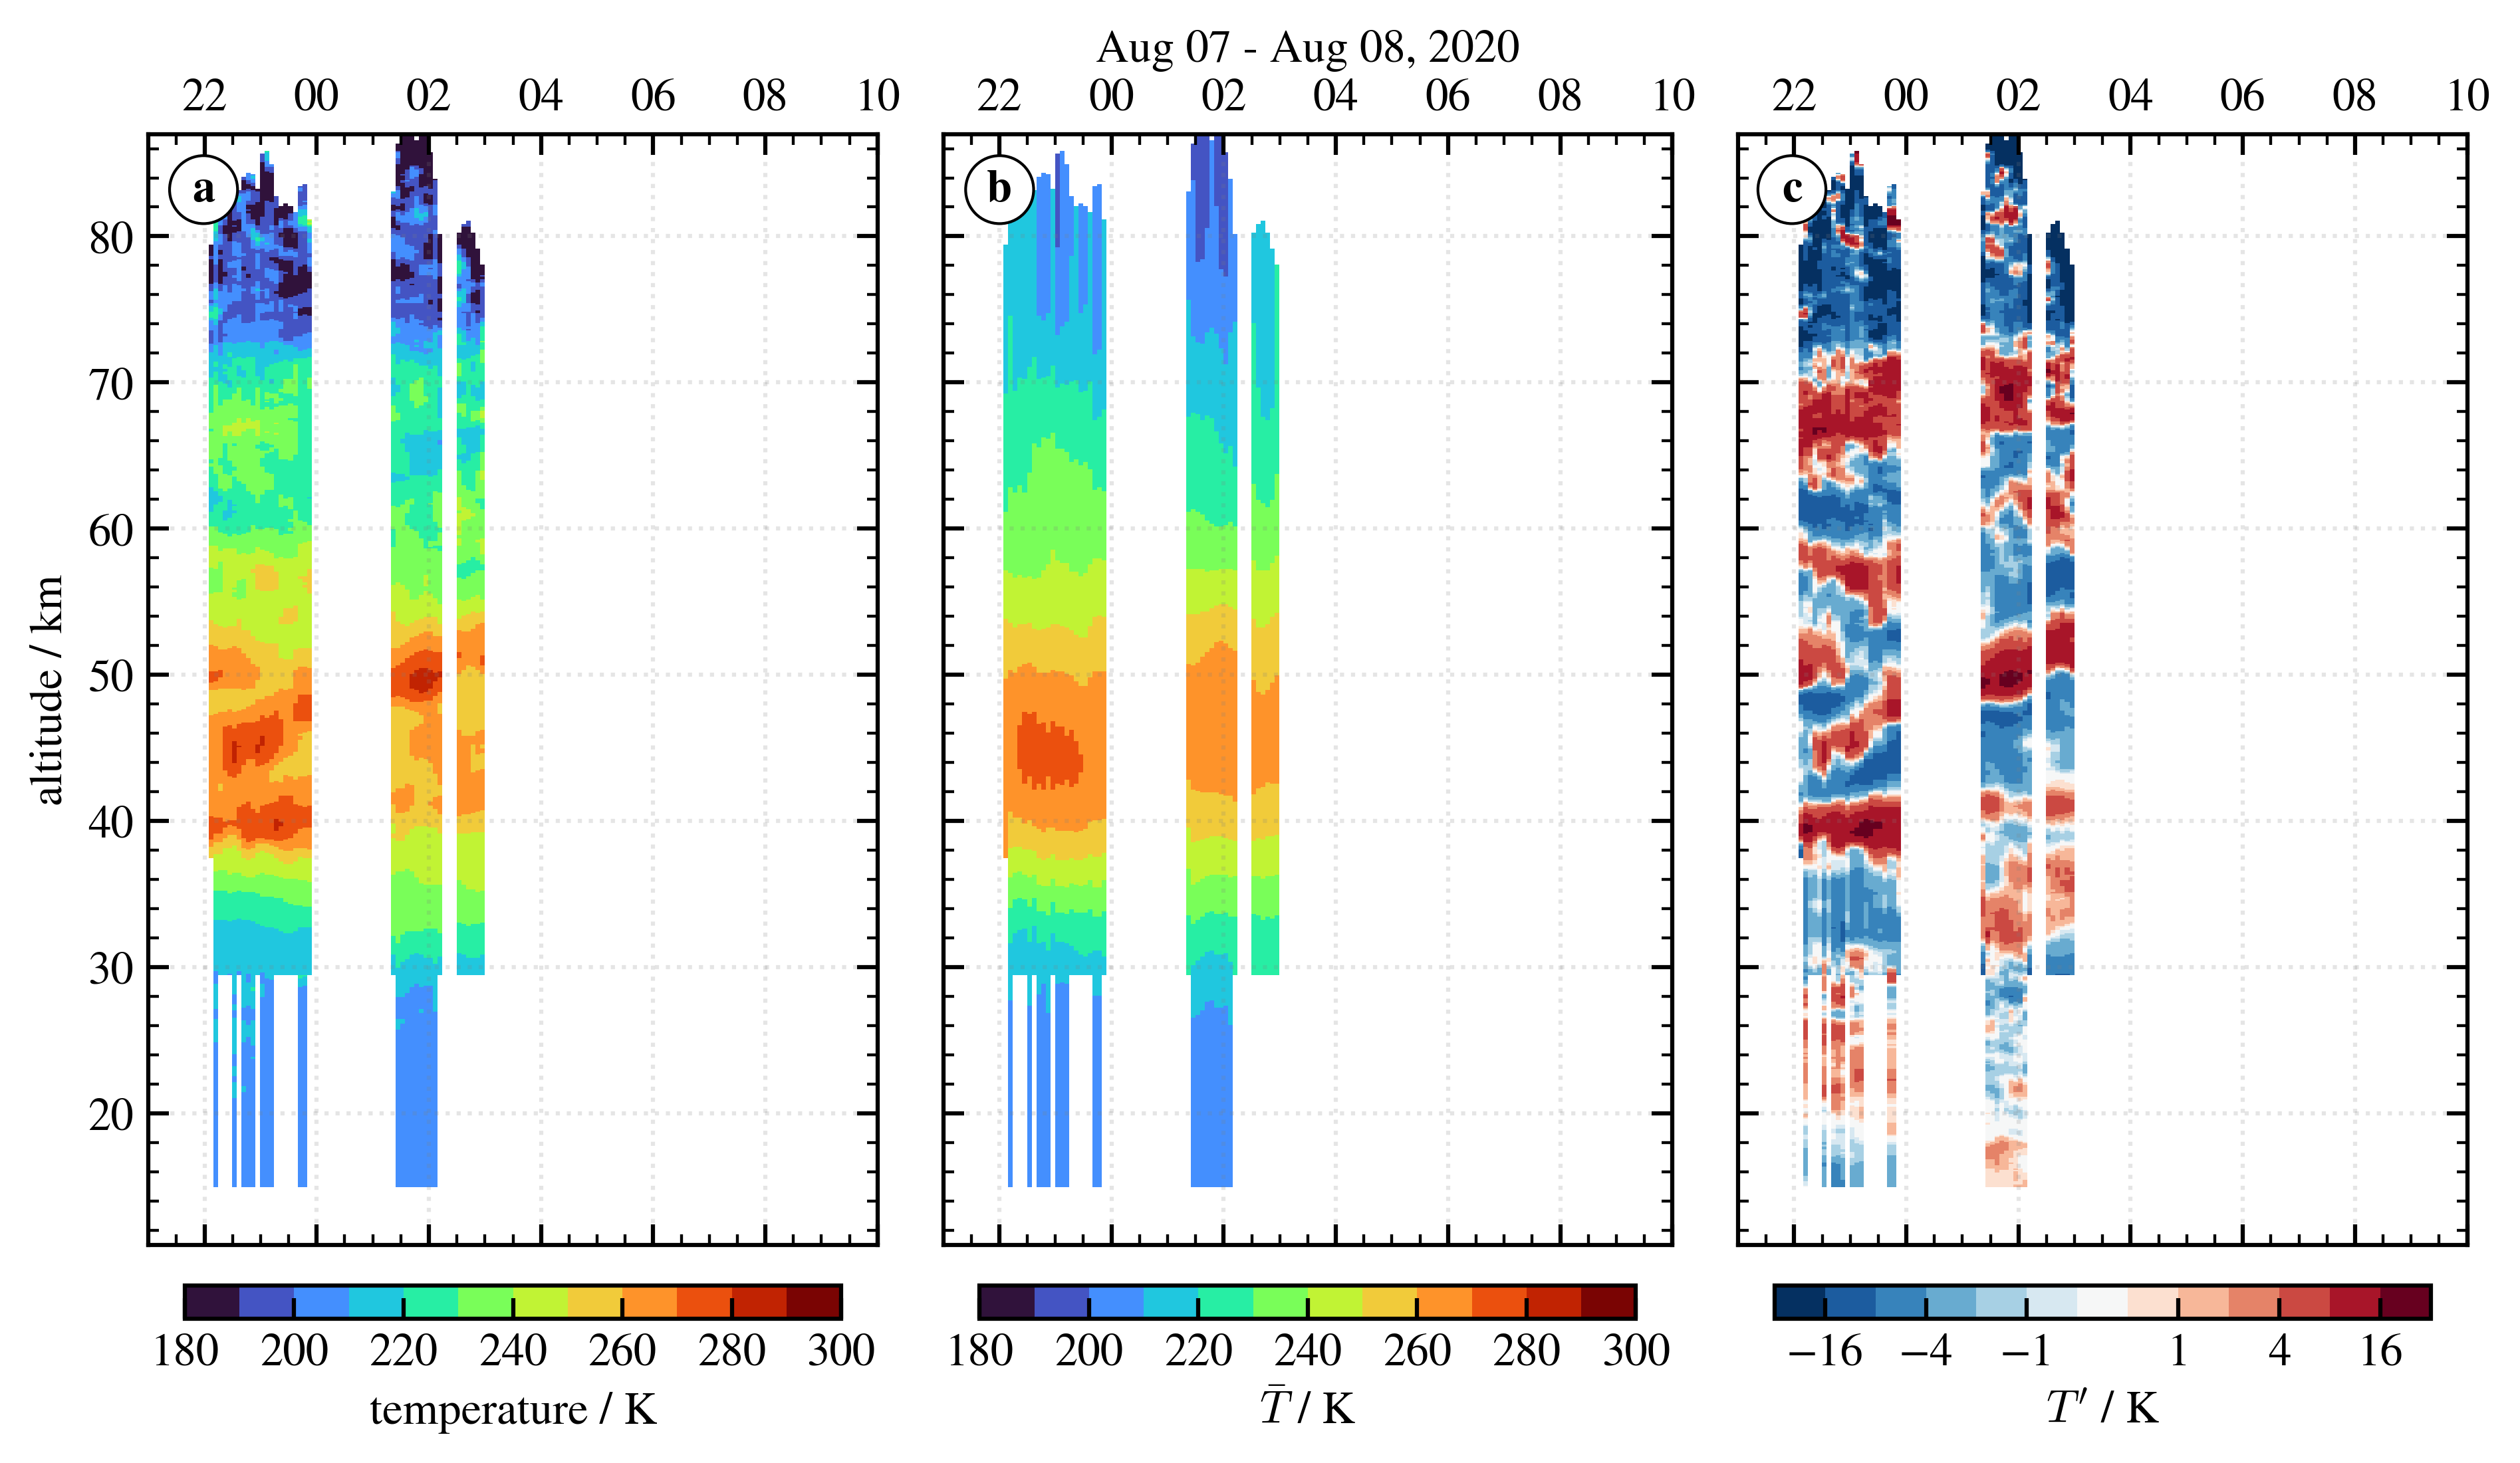
\includegraphics[width=0.9\textwidth]{figures_lidar/coral_event_20200807.png}
    \caption{Identical to Figure \ref{fig:coral_2018} showing night-time measurements from the 7th to the 8th of August 2020. Periods of missing data are related to cloud coverage.}
    \label{fig:coral_2020}
\end{figure*}
In the first measurement (Figure \ref{fig:coral_2018}c), upward tilted phase lines are clearly observed after 05:00$ \, \mathrm{UTC}$. Horizontal phase lines before 05:00$ \, \mathrm{UTC}$ might indicate that these waves are related to a MW event with non-stationary processes, but a more detailed analysis of the synoptic situation is essential for further interpretations. The same is true for the second observation. Again Figure \ref{fig:coral_2020}c shows upward tilted phase lines which are most pronounced between 40 and \SI{60}{\kilo\meter}. Unfortunately, this night was temporarily cloudy at Río Grande preventing a continuous measurement, but it might as well be promising, if these clouds are related to a passing frontal system and a tropopause fold on the larger scale. To support further interpretations of the measurements concise overviews of corresponding ERA5 data follow.

Similar figures (Figure \ref{fig:era5_2018} and \ref{fig:era5_2020}) are presented for both CORAL measurements that try to reproduce the measurements in the ERA5 data (a), visualize GW activity in the stratosphere (b and c) and corresponding dynamics at tropopause level (d, e and f). In addition, wind and geopotential height at \SI{850}{hPa} in (f) provide an idea on the prevailing forcing conditions for MWs in the same figure. \\
Phase lines in both vertical timeseries (a) agree well with the measurements of CORAL. The waves' phases match with the overlayed measurements and the phase lines also tilt upward for the measurement periods. It strongly suggests that the processes that lead to the upward tilt in both CORAL measurements are represented in ERA5 and sufficiently covered in the dynamics of the underlying IFS model. Taking a closer look at each case can be instructive.
%%% Is ERA5 based on 9km IFS model runs???
%%% - state that vertical time series would look quite similar to observations - angle of idealized simulation for realistic wind profile -> approximately 20km / 12h 

\subsection*{ERA5 overview for June 22nd/23rd, 2018 measurements}
\begin{figure*}[tbp]
    \centering
    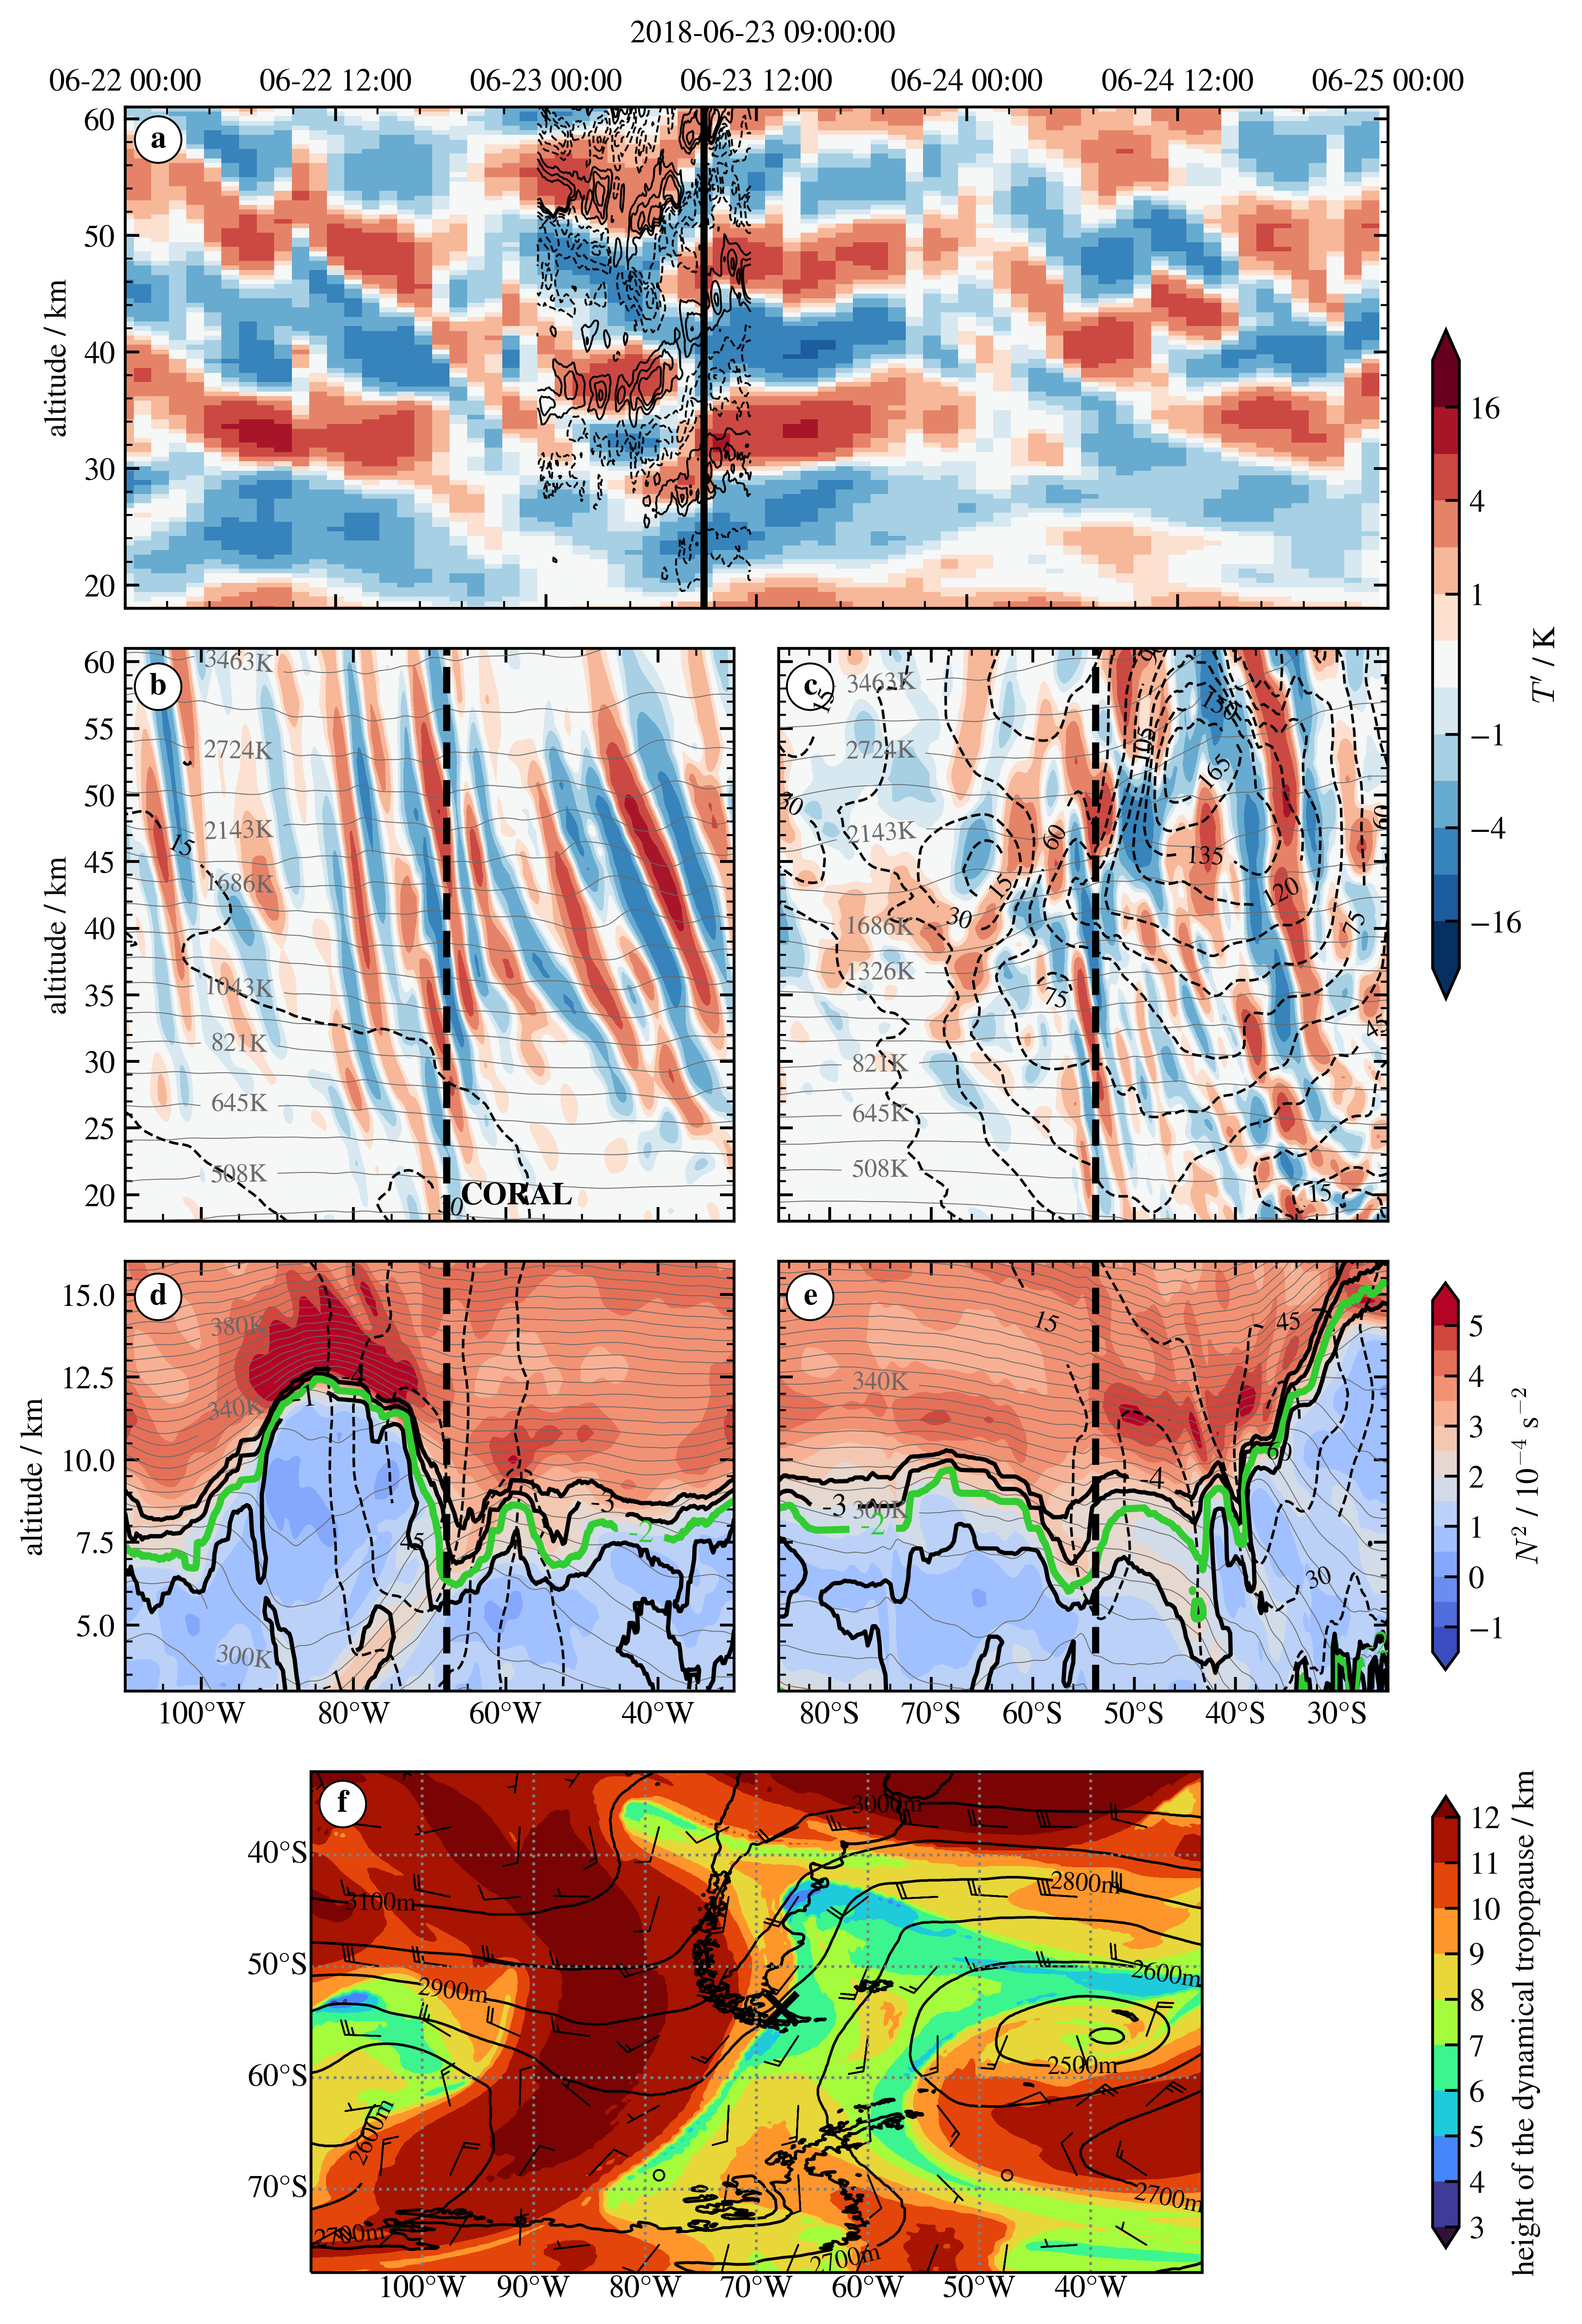
\includegraphics[width=0.75\textwidth]{figures_lidar/era5_trop_strat_33.png}
    \caption{ERA5 overview for the first CORAL measurement from the 22nd to the 23rd of June 2018. (a) shows vertical profiles of stratospheric temperature perturbations for CORALs location after applying a vertical butterworth filter similar to the measurements (Figure \ref{fig:coral_2018}c). The measurement itself is overlayed by thin black lines (dashed lines represent negative values). (b) and (c) show vertical cross sections of stratospheric temperature perturbations (after applying a horizontal Gaussian filter) for the latitude (b) and longitude (c) of CORAL. (d) and (e) show corresponding vertical cross sections at tropopause level with thick lines indicating PVU levels 1-4 (2 in green) and $N^2$ color coded to differentiate between tropospheric and stratospheric air. Dashed lines in the vertical cross sections show zonal ((c) and (e)) and meridional ((b) and (d)) winds. (f) shows the height of the dynamical tropopause in a horizontal cross section for the \SI{2}{PVU} level color coded with geopotential height and wind barbs for the \SI{850}{hPa} level. The vertical line in (a) marks the time for (b)-(f).}
    % The vertical line in (a) marks the time for (b)-(f) and CORAL's location is highlighted in the vertical cross-sections (b)-(e) and with a cross in (f).
    \label{fig:era5_2018}
\end{figure*}
At first, we want to find out if a tropopause fold could be the reason for the upward tilted phase lines in Figure \ref{fig:coral_2018}c. The vertical cross sections at tropopause level (Figure \ref{fig:era5_2018}d and e) show vanishing structures of a tropopause fold, but preceding timestamps clearly illustrate that the fold's core already passed CORAL \SI{24}{h} earlier. Blue colors northeast of CORAL in (f) indicate the position of the fold during the observations, too. Signatures of upward tilted phase lines in the extended vertical timeseries (Figure \ref{fig:era5_2018}a) and in the measurements appear significantly after the passage of the fold. It appears that in this case the upward tilted phase lines are not caused by NOGWs above a propagating tropopause fold. Can alternative processes be identified in the ERA5 data?

During the observation a strong negative PV anomaly (centered around \SI{85}{\degree W} in (d)) with a substantial warm air mass below (dark red area in (f)) approaches CORAL. On the southern hemisphere warm air advection is accompanied by wind backing, which can be observed in (f) over multiple timesteps, too. The large scale wind direction around CORAL changes from south to southwest at lower levels resulting in a transient wind forcing. It then transitions into a quite stationary regime favoring the excitation of MWs at the southernmost mountain range of the Andes, the Cordillera Darwin. The vertical timeseries in (a) supports this interpretation. The upward tilted phase lines transition into horizontal phase lines that persist for almost \SI{12}{h} subsequent to the period of the CORAL measurements. A clear sign for stationary MWs. In addition, phase lines in (b) and (c) around \SI{20}{\kilo\meter} and above indicate the propagation of MWs excited southwest of CORAL's location, too.

All in all, these observations in the ERA5 data draw a conclusive picture and suggest that the upward tilt of phase lines in the first CORAL measurement (Figure \ref{fig:coral_2018}c) is caused by a transient wind forcing with wind backing that results in non-stationary MWs. 
%% for about \SI{6}{h}.
%% exceptionally strong PNJ with significant shift of PNJ to the north for that point in time
%% check spacing of paragraphs of proposal
%% apparently
\subsection*{ERA5 overview for August 7th/8th, 2020 measurements}
\begin{figure*}[tbp]
    \centering
    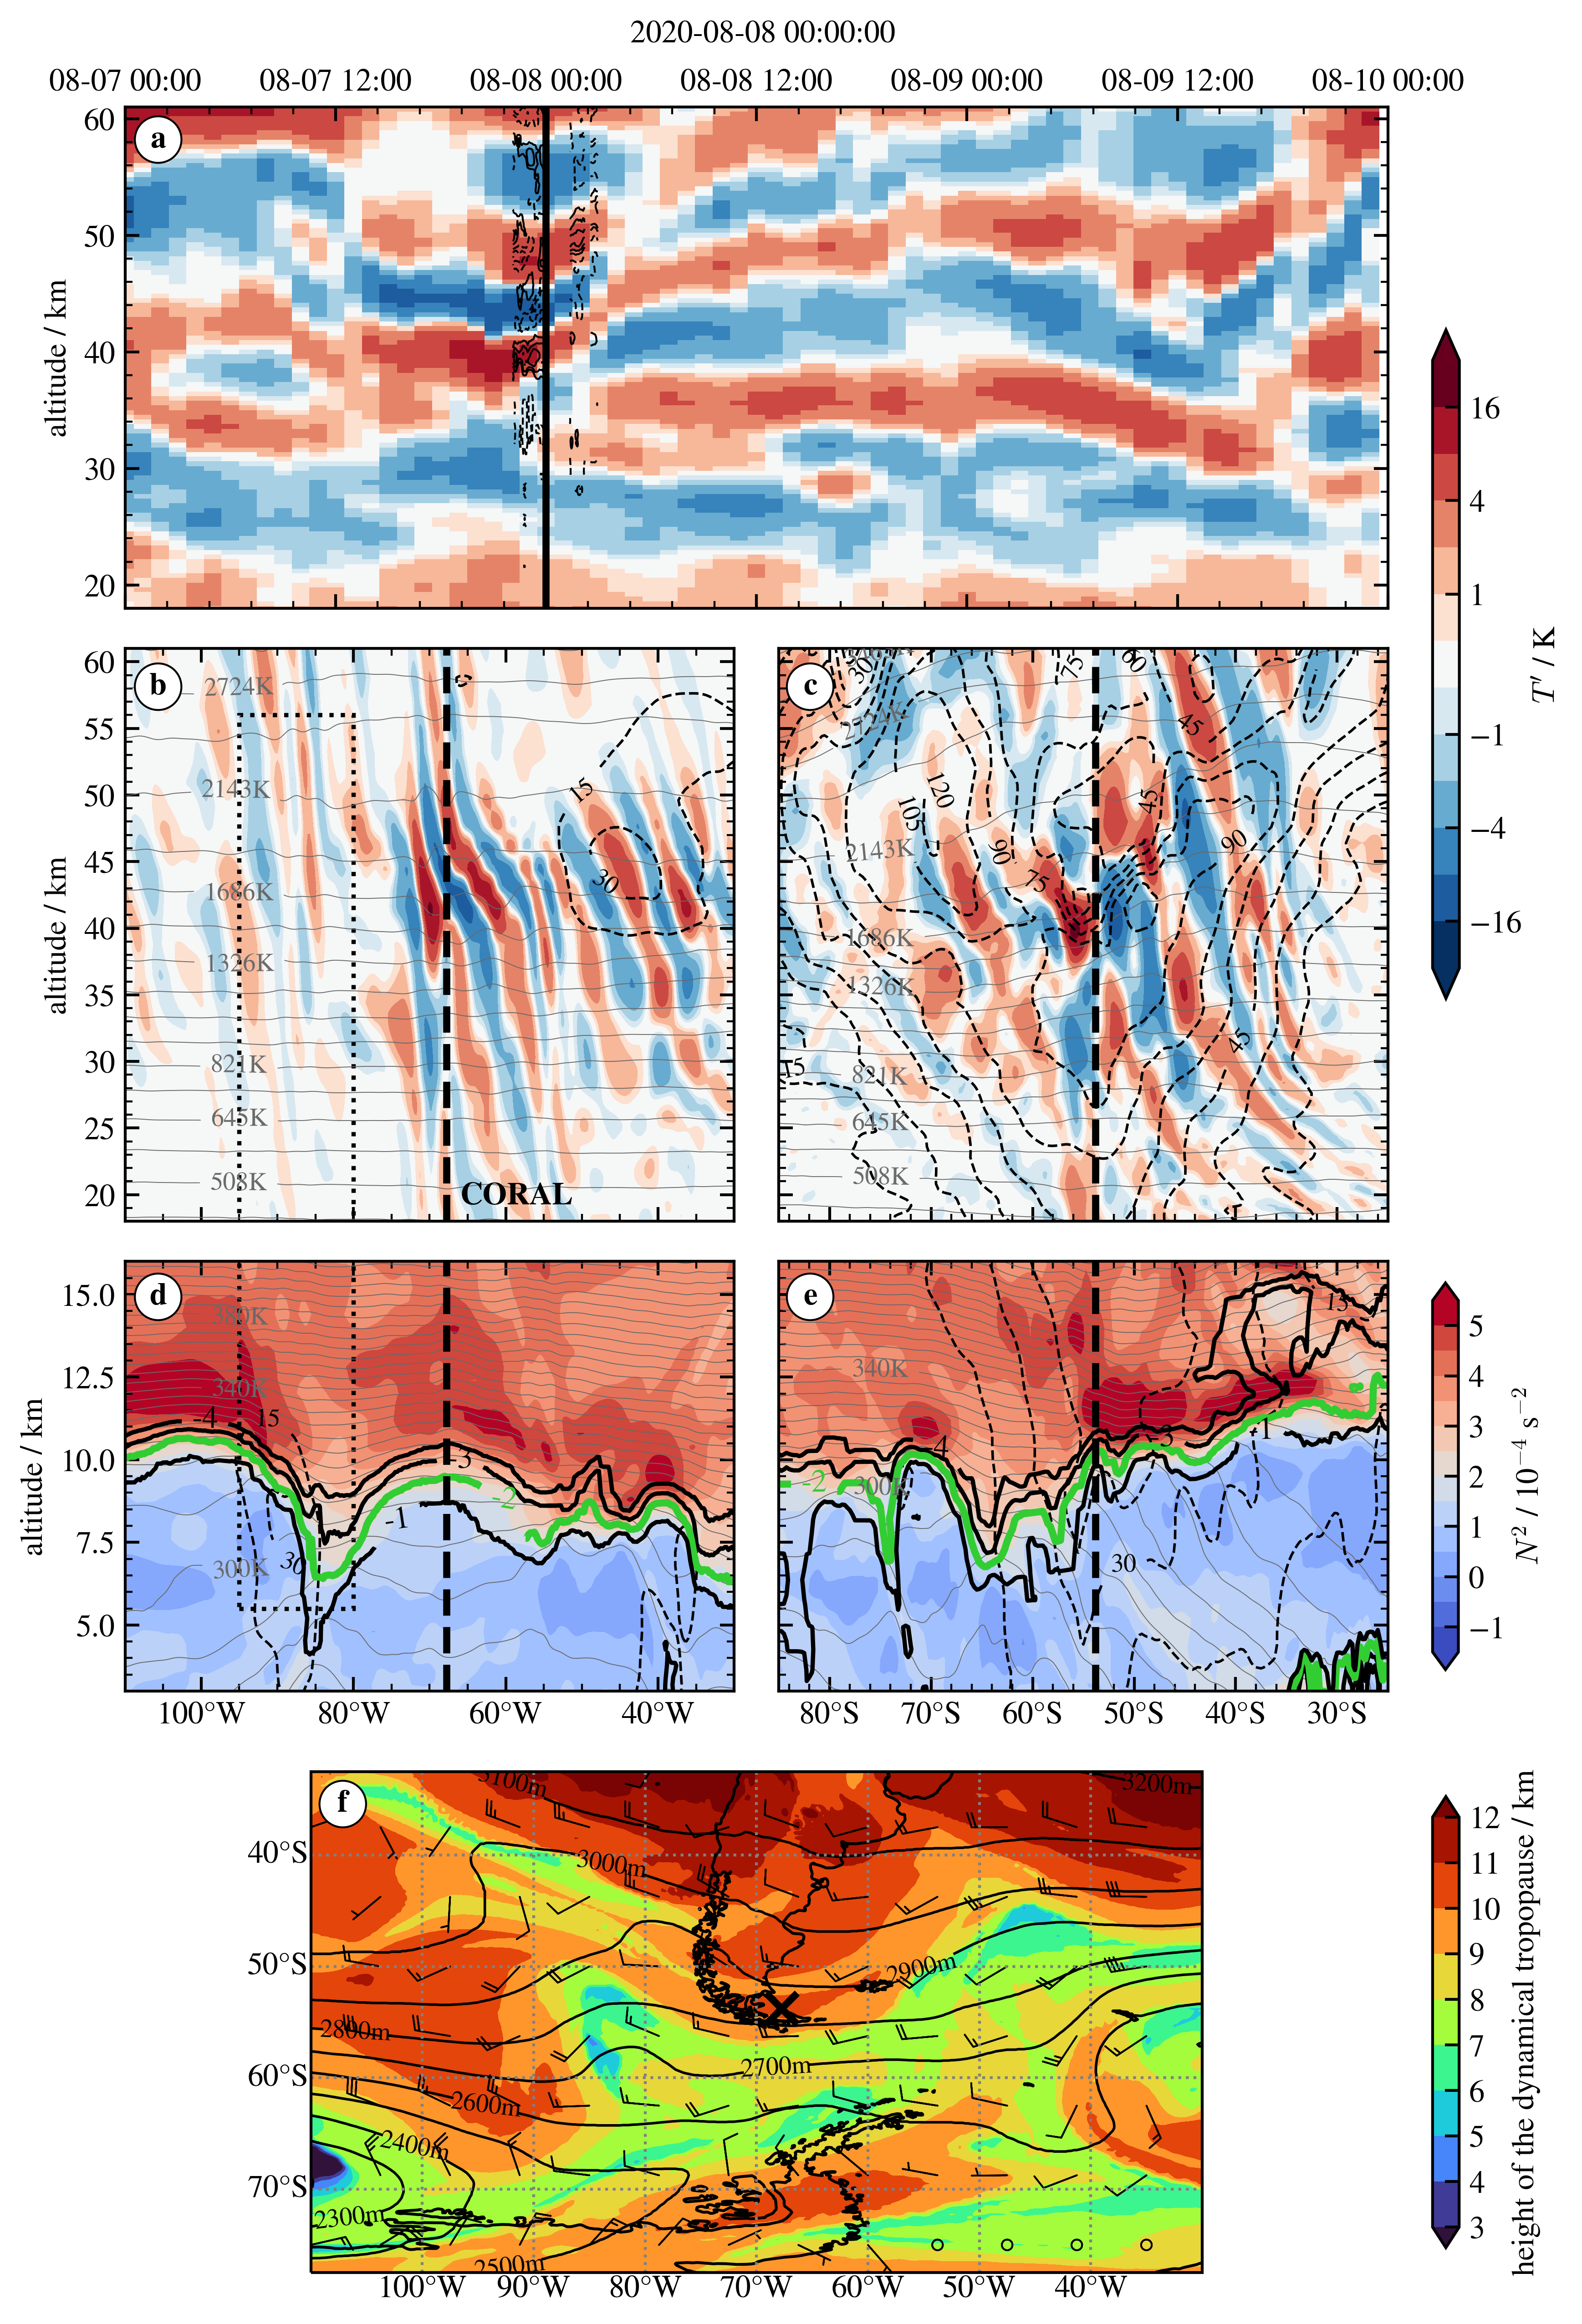
\includegraphics[width=0.8\textwidth]{figures_lidar/era5_trop_strat_24.png}
    \caption{Identical to Figure \ref{fig:era5_2018} showing an overview of ERA5 data for the second CORAL measurement from the 7th to the 8th of August 2020. The dotted rectangle in (b) and (d) frames GWs in the stratosphere above a tropopause fold west of CORAL's location over the Pacific Ocean.}
    \label{fig:era5_2020}
\end{figure*}
Again, we first check for the presence of a tropopause fold during the CORAL observation. The PVU levels in (d) and greenblue colors in (f) of Figure \ref{fig:era5_2020} indicate the development of a textbook tropopause fold west of CORAL at \SI{85}{\degree W} (more details in next subsection), but once more, the timing of its pass over CORAL does not fit to the measurements. The significant upward tilt of phase lines in (a) between approximately 21:00 and 04:00$ \, \textrm{UTC}$ appears earlier than the pass of the depression around 17:00$ \, \textrm{UTC}$ on the 8th of August. Could a transient wind forcing explain the upward tilt once again?

As depicted in the meridional cross section (c), the PNJ is centered directly above CORAL for this event. Considering the horizontal refraction of GWs into the jet discussed in chapter \ref{sec:results3D}, phase lines observed in the extended vertical timeseries in (a) at higher alitudes might actually belong to sources further north or south. Phase lines in (c) suggest that waves observed with CORAL above \SI{40}{\kilo\meter} originate further north from latitudes around 40-\SI{50}{\degree S}. The Andes Mountains align nearly exactly in a north-south direction in this latitude band and are a reliable source for MWs. In fact, the direction and speed of the prevailing wind in (f) that flows over the Andes in that area changes its direction before and during the period of the observations. Speed increases and the wind transitions from a westerly to a more northwesterly flow (wind veering like in the first event). However, conditions are not as distinct as in the first case. Wind speed and direction at lower levels continue to change afterwards and another feature in the ERA5 data should be noted.

Meridional winds in (b) show a wind veering from a westerly towards a more southwesterly flow between 40 and \SI{60}{\kilo\meter} and 35 to \SI{50}{\degree W}. This meandering of the PNJ passed CORAL around 19:00$ \, \textrm{UTC}$, so just three hours before CORAL started its measurements. When observing the phase lines in (b) for multiple timesteps a compression of the vertical wavelengths can be observed, which seems to follow the meandering of the PNJ. This fits to the upward tilted phase lines in (a). The vertical wavelengths decrease towards the end of the upward tilt before they increase again.

In conclusion, the interpretation of the ERA5 data is not as clear for the second CORAL measurement. GWs above a propagating tropopause fold can be ruled out as the source for the upward tilted phase lines, but alternative processes are not fully conclusive, too. Nevertheless, it is likely that transient wind conditions close to the ground which relate to the forcing conditions and transient conditions of the PNJ are the reason for the phase line's upward tilt.
% With some imagination phase lines still turn upward...

\subsection*{NOGWs above a tropopause fold over the Pacific Ocean}
The dotted rectangle in (b) and (d) of Figure \ref{fig:era5_2020} frames GWs in the stratosphere above a tropopause fold that are already visible in the lower stratosphere and very similar to GWs in the ERA5 analysis in Figure \ref{fig:RF25_era5_vertical} by \textcite{dornbrack_stratospheric_2022}. The connection of these GWs to the tropopause fold below becomes even clearer in the attached animation. Preceding and subsequent timesteps also display GWs above this tropopause depression and show how these waves propagate with the depression underneath. In addition to the case study by \textcite{dornbrack_stratospheric_2022}, it represents another ERA5 example of NOGWs above a propagating tropopause depression that emulate the pattern of MWs. \\
Here, the depression propagates over the Pacific Ocean, so its vicinity to the southern tip of South America allows a direct comparison of these waves to the MWs over the Andes in Figure \ref{fig:era5_2020}b. Maximum amplitudes of NOGWs above the Pacific ($\approx \SI{4}{K}$ between 40 and \SI{45}{\kilo\meter}) are significantly lower than amplitudes at the same time and latitude over the Andes mountains ($\approx \SI{16}{K}$ between 40 and \SI{45}{\kilo\meter}). This is consistent with the climatological analysis of AIRS satellite observations in Figure \ref{fig:hindley_2020_GWMF} that reveals significantly smaller momentum fluxes for NOGWs over the ocean (\cite[]{hindley_18year_2020}), but it can also complicate the detection of these NOGWs in ground-based lidar measurements at locations which are superposed by MWs as in CORAL's case. At these locations, the isolation of NOGWs in the measurements are probably cumbersome and not always possible. \\
On the other hand, phase lines of GWs in both regions in Figure \ref{fig:era5_2020}b show a comparable pattern and lean into the predominantly westerly flow. It consolidates the hypothesis that a tropopause depression could be an obstacle to the stratospheric flow aloft, similar to mountains at the surface. 
% It suggests a comparable excitation process.

\section{Summary and answer to research question (R5)}
\label{sec:lidOb-summary}
This chapter focused on relating the theoretical foundations from previous chapters to potential measurements in the real atmosphere. More specifically, the goal was to utilize the idealized numerical simulations of this work to identify patterns of NOGWs from propagating tropopause folds in lidar measurements to answer the last research question of this thesis:
%
\begin{tcolorbox}[]
    (R5) Can NOGWs from propagating tropopause depressions be identified in ground-based lidar observations?
\end{tcolorbox}
%
Vertical timeseries were presented which mimic the measurement of a ground-based lidar in the idealized simulations. These showed a clear pattern for GWs from a propagating source (e.g. a tropopause fold) with upward tilted phase lines. The angle of the tilt depends on the propagation speed of the source and the horizontal wavelength of the GW. Thus, it should be possible to detect NOGWs from propagating tropopause folds in lidar observations from a theoretical point of view.

In a next step, we checked measurements of the lidar system CORAL from the southern tip of South America and presented two observations that include the pattern of upward tilted phase lines in the lidar data. However, upward tilted phase lines in vertical timeseries can not only result from a progating GW source. Other processes that result in a similar pattern are for example downward propagating GWs or transient atmospheric conditions during the excitation or propagation of the GWs. Therefore, corresponding ERA5 data was analysed to pinpoint the processes that led to the signatures in the measurements. \\
The analysis revelead that tropopause folds were not causing the upward tilted phase lines in both case studies, but transient background conditions and MWs. In addition, a comparison of NOGWs above a tropopause fold over the Pacific Ocean to MWs over the Southern Andes showed that the amplitudes of these NOGWs are approximately a factor 4 smaller than amplitudes of MWs over the Andes. It might be difficult to isolate these NOGWs in the lidar measurements at locations that are generally dominated by strong MW events like CORAL. Most likely, a lidar location less influenced by MWs could reveal if the discussed signatures can be identified above propagating tropopause folds and provide further insights on the proposed excitation process in the real world.

To conclude, theory and idealized numerical simulations present a clear pattern of NOGWs from propagating tropopause folds that can be identified in observations. In practice though, it can be challenging to relate these signatures of GWs in lidar measurements to explicit processes in the real atmosphere. Additional information from models is needed and, up to today, it was not possible to link ground-based lidar measurements to NOGWs above tropopause folds and confirm the excitation process suggested by \textcite[]{dornbrack_stratospheric_2022}.
%% Overall conclusion:
% No matter what the escitation process for NOGWs is, they would be much easier derived in lidar data far away from orography, because the superposition with MWs can be ruled out.
% Waves can be observed in vertical cross section above tropopause fold in era5 like in doernbrack paper
% theoretically yes - practically not confirmed
% include characterisation of NOGWs from folds in research question????